Esta sección detalla en profundidad los paquetes de autenticación utilizados en sistemas basados en Windows. Los paquetes de autenticación son {\it Dynamic-Link Libraries (DLLs)} lanzadas por el proceso LSA durante un inicio de sesión que se encargan de analizar y validar las credenciales introducidas por el usuario, crear una nueva {\it logon session} y pasar la información al proceso LSA para que este cree el {\it Access Token} correspondiente si la validación ha sido correcta. Windows permite la carga de multiples paquetes de autenticación lo que permite que LSA siporte multiples procesos de inicio de sesión diferentes. En este capítulo se van a detallar los paquetes de autenticación utilizados por defecto: MSV1\_0 y Kerberos. Además, se va a detallar la forma que tiene Windows de almacenar las contraseñas en el sistema.

\section{MSV1\_0}

MSV1\_0~\cite{Capitulo3:MSV10} es el paquete de autenticación proporcionado por Windows e implementa la familia de protoclos Lan Manager versión 1 y 2 (LM y NT) y Net Lan Manager versión 1 y 2 (NTLMv1 y NTLM v2)~\cite{Capitulo3:NTLM}. \\

Este paquete de autenticación soporta tanto inicio de sesión de forma local como inicio de sesión para cuentas y servicios en dominios. El paquete MSV1\_0 ejecuta una aquitectura cliente/servidor, es decir, el cliente es el que recibe las credenciales (username y el hash de la contraseña) y las valida frente al servidor. \\

Cuando se ejecuta localmente cliente y servidor están representados por la misma máquina que se encarga de recoger las credenciales proporcionadas por el usuario a través de los {\it Credential Providers} y compararlas con las credenciales introducidas por el usuario cuando creó la cuenta y que están almacenadas en la SAM, si ambas contraseñas son iguales el proceso de autenticación es correcto. \\

En inicio de sesión en dominio el cliente representa la máquina local y el servidor representa el Domain Controller donde está configurado Active Directory. El cliente recoge las credenciales y las pasa por el canal de comunicación seguro creado por el proceso {\it Winlogon.exe} y las comunica con la instancia de MSV1\_0 ejecutada en el Domain Controller. El cliente delega la comprobación de las credenciales al Domain Controller, esto se denomina {\it Pass-Through}. La instancia de MSV1\_0 del Domain Controller realiza la validación de las credenciales comprobando la información recibida con los datos almacenados el la base de datos del Domain Controller y devuelve la información a la instancia ejecutada en local. Si la validación ha sido correcta, el paquete MSV1\_0 local devuelve la información al proceso LSA local. \\

Windows ha implementado los protocolos de desafío/respuesta NTLMv1 y NTLMv2 para la intercambiar las credenciales introducidas por el usuario entre la máquina local y el Domain Controller en lugar de intermbiar las credenciales directamente. Antes de detallar ambos protocolos, se va a analizar la forma de almacenamiento de las contraseñas que luego serán utilizadas por ambos protocolos. 


\subsection{Windows hashes}

Los Sistemas Windows, en lugar de almacenar las contraseñas en texto plano, algo que sería un gran problema de seguridad utilizan los siguientes algoritmos de hash~\cite{Capitulo3:Hashes}:

\subsubsection{Hashes Lan Manager (LM)}

El algoritmo Lan Manager (LM) para realizar la función hash de las contraseñas almacenadas en Windows fue una de las primeras implementaciones que desarrolló Windows para mantener cifradas las contraseñas. Hoy en día está práctiacamente en desuso y desde 2017 se recomienda desactivar la opción de que se guarden las credenciales de esta forma~\cite{Capitulo3:LMDeprecated}. 

\textbf{Algoritmo}

El algoritmo de hash utilizado realiza el siguiente procedimiento: 

\begin{itemize}
\item Convertir todos los carácteres a letras mayúsculas.
\item Añadir un padding de carácteres nulos hasta que tenga una longitud de 14 carácteres. 
\item Dividir la contraseña en dos partes de 7 carácteres cada una. 
\item Crear dos DES keys para cada parte. 
\item Cifrar a través de DES las partes anteriores con el string "KGS!@\#\$\%".
\item Concatenar ambos strings.
\end{itemize}

\subsubsection{Hashes NT}

Los hashes NT, también conocidos como hashes NTLM, es la forma que utiliza atualmente Windows para alamcenar las contraseñas de los usuarios del sistema. Estos hashes están almacenados en la SAM si se trata de un equipo local o en el fichero NTDS del Active Directory si se trata de un equipo en dominio. A través de la obtención de este tipo de hashes se puede realizar un ataque de Pass-The-Hash (se detallara en los siguientes capítulos).

\textbf{Algoritmo}

Windows encodea la contraseña del usuario con UTF-16 Little Endian y posteiormente realiza un hash con el algoritmo MD4: 

\begin{itemize}
\item MD4(UTF-16-LE(password))
\end{itemize}

\subsection{Net-NT Lan Manager (Net-NTLM)}

El protocolo Net-NTLM es un protocolo {\it challenge/response} utilizado para la autenticación entre el cliente y el servidor~\cite{Capitulo3:NTLM2}. El objetivo principal de este protocolo es proporcionar la autenticación de un dispositivo sin la necesidad de intercambiar implícitamente la contraseña con el servidor. Además, este protocolo proporcionada integridad y confidencialidad ya que los mensajes intercambiados van cifrados. Windows ha proporcioado dos implementaciones de este protocolo~\cite{Capitulo3:NTLANManager}:

\subsubsection{Net NT Lan Manager Versión 1 (Net-NTLMv1)}

Es la versión más antigua de este protocolo y actualmente se encuentra en desuso ya que presenta limitaciones de gran importancia. Este protocolo utiliza ambos de los hashes explicados en la sección anterior (LM y NT). A continuación se va a detallar protocolo utilizado:

\begin{enumerate}
\item El cliente realiza una petición de autenticación al servidor.
\item El servidor responde con un challenge que corresponde a un número aleatorio de 8 bytes. 
\item El cliente realiza una operación criptográfica utilizando el challenge enviado por el servidor y un secreto que ambos conocen, en este caso se va a utilizar alguno de los windows hashes explicados anteriormente (o los dos). El cliente enviará al servidor el resultado de esta operación (24 bytes). 
\item El servidor comprueba si se ha realizado la operación correctamente ya que también dispone tanto el challenge como el secreto utilizado. Si el challenge coincide la autenticación se ha realizado correctamente. 
\end{enumerate}

\subsubsection{Net NT Lan Manager Versión 2 (Net-NTLMv2)}

Debido a las limitaciones que presentaba NTMLv1, Windows implementó una versión mejorada de este protocolo: NTLMv2 que está disponible desde el paquete Windows NT 4.0 SP4. De la misma manera, se va a explicar el protocolo {\it challenge/response} utilizado para esta versión:

\begin{enumerate}
\item El cliente realiza una petición de autenticación al servidor. 
\item El servidor responde con un challenge que corresponde a un número aleatorio de 8 bytes.
\subitem - Server Challenge (SC) = 8-byte challenge (Random).
\item El cliente genera también un numbero aleatorio de 8 bytes.
\subitem - Client Challenge (CC) = 8-byte challenge (Random).
\item El cliente calcula el secreto que va a utilizar a través de realizar el algorimo HMAC-MD5 del hash NT de la contraseña, el nombre de usuario y el dominio. 
\subitem v2-Hash = HMAC-MD5(NT-Hash, user name, domain name)
\item El cliente envía dos respuestas diferentes: 
\subitem - LMv1: Que corresponde con el hash HMAC-MD5 del v2-hash y los dos challenges (SC y CC): LMv2 = HMAC-MD5(v2-Hash, SC, CC)
\subitem - NTv2: Que corresponde con el hash HMAC-MD5 del v2-hash, el challenge del sevidor y un nuevo challenge del cliente que incluye un timestamp para evitar ataques de replay: CC* = (X, time, CC2, domain name) --- NTv2 = HMAC-MD5(v2-Hash, SC, CC*)
\item El servidor comprueba si se las operaciones se han realizado correctamente ya que también dispone tanto el challenge como el secreto utilizado. Si el challenge coincide la autenticación se ha realizado correctamente.
\end{enumerate}

\section{Kerberos}

El paquete de autenticación Keberos, que implementa la versión 5 del protocolo de Kerberos~\cite{Capitulo3:Kerberos}, es el paquete principal utilizado por los sistemas Windows para verificar la identidad de un equipo cuando se realiza un inicio de sesión en red. Las principales características de este protocolo son~\cite{Capitulo3:Kerberos2}: 
\begin{itemize}
\item Proporcionar autenticación a través del uso de tickets.
\item Evitar el intercambio o almacenamiento de credenciales. 
\item La utilización de un tercero de confianza ({\it trusted 3rd-party}).
\item La utilización de criptografía simétrica. 
\end{itemize}

\subsection{Aplicaciones de Kerberos}

Las ventajas de utilizar Kerberos como protocolo de autenticación son las siguientes~\cite{Capitulo3:Kerberos3}:

\begin{itemize}
\item \textbf{Autenticación delegada:} La autenticación con Kerberos permite a un servicio actuar impersonando al cliente local cuando se conecta a otros servicios.
\item \textbf{Single Sig-On:} El uso de Kerberos permite a los usuarios acceder a los recursos de un dominio sin introducir la contraseña cada vez que quieran acceder a un recurso diferente.
\item \textbf{Autenticación eficiente:} El servidor donde se está intentado loguear un equipo tiene la capacidad de autenticar a este examinando únicamente las credenciales presentadas por el cliente. Es decir, un cliente puede obtener las credenciales para un servidor en partciular una vez y reutilizarlas. 
\item \textbf{Autenticación mutua:} A diferencia de NTLM, Kerberos puede autenticar ambas partes, tanto el cliente como el servidor. 
\end{itemize}

\subsection{Elementos principales}

Antes de explicar el procedimiento utilizado por el paquete de autenticación Kerberos, es necesario detallar los diferentes elementos que van a formar parte del mismo~\cite{Capitulo3:Kerberos4}. 

\subsubsection{Ticket-Granting Ticket (TGT)}

{\it Ticket-Granting Ticket (TGS)} corresponde con un identificador cifrado con un tiempo de uso limitado expedido por el Key Distribution Center (KDC) cuando se ha completado la autenticación de un usuario y sirve para solicitar los {\it Ticket-Granting Server (TGS)} cuando se quiere utilizar dicho servicio. Este ticket está cifrado con la clave del KDC. El tiempo de validez por defecto de un ticket es de diez horas. 

\subsubsection{Ticket-Granting Server (TGS)}

{\it Ticket-Granting Server (TGS)}~\cite{Capitulo3:TGT} es el identificador que un usuario presenta a un servicio para poder acceder a sus recursos. Para solicitar este ticket el usuario presenta el {\it Ticket-Granting Ticket (TGS)} para verificar la validez de la autenticación y si tiene permisos de acceso a este recurso. Este ticket etá cifrado con la clave del servicio correspondiente.

\subsubsection{Key Distribution Center (KDC)} 

{\it Key Distribution Center (KDC)} es el servicio encargado de recibir las peticiones de autenticación, validar los datos contenidos en esta y si la autenticación es correcta proporcionar un {\it Ticket-Granting Ticket (TGT)}. Este proceso se ejecuta en el Domain Controller que administra el Active Directory. \\

Este elemento se puede dividir en dos instancias principales: El servidor de autenticación ({\it Authentication Server}) y el servidor que gestiona los TGTs ({\it Ticket Granting Server}). 

\begin{itemize}
\item \textbf{Authentication Server (AS):} Proporciona la autenticación de un usuario en la red y genera el ticket TGT. 
\item \textbf{Ticket Granting Server (TGS):} Cuando un usuario solicita el acceso a un servicio red, presenta el ticket TGT y este le proporciona un ticket TGS que sirve de autenticación frente al servicio de red destino. 
\end{itemize}

\subsubsection{Application Server (AP)}

{\it Application Server (AS)} corresponde con cualquier aplicación que soporte autenticación a través del protocolo Kerberos. Corresponde al servicio o recurso al que quiere acceder el cliente. 

\subsubsection{Claves}

En el protocolo de autenticación Kerberos hay tres claves fundamentalmente: 
\begin{itemize}
\item \textbf{Clave del KDC o krbtgt:} Clave derivada del hash NTLM de la cuenta {\it krbtgt}, sirve para cifrar las partes más importantes del protocolo como el TGT.
\item \textbf{Clave del cliente: } Clave derivada del hash NTLM del usuario o cliente. 
\item \textbf{Clave del servicio: } Esta clave depende del servicio y es la que se utiliza para cifrar los tickets TGS. 
\end{itemize}

También existen diferentes claves de sesión negociadas entre el KDC y el cliente y claves de sesión del servicio negociada entre el cliente y el AS. 

\subsubsection{Privilege Attribute Certificate (PAC)}

{\it Privilege Attribute Certificate (PAC)}~\cite{Capitulo3:PAC} es una estructura de datos que recoge la información codificada sobre los privilegios del usuario. Esta estrucura está cifrada con la clave del KDC. El cliente puede especificar que no se incluya el PAC en la petición del TGT. Un servicio puede comprobar con el KDC si el PAC está firmado correctamente. 

\subsection{Protocolo de autenticación}

En esta sección se va a explicar el protocolo de autenticación, para este caso de usuo el cliente solicita un TGT para autenticarse y posteriormente utiliza ese TGT para pedir un ticket de servicio para poder acceder a una aplicación. Se va a detallar el proceso utilizado y los paquetes intercambiados~\cite{Capitulo3:Kerberos5}. Cabe destaca que Kerberos utiliza  TCP y UDP para el intercambio de paquetes. El KDC utiliza los puertos TCP/88 y UDP/88.   

\begin{figure}[t!] %[ht!] para here [b] para bottom [t] para top
\begin{center}
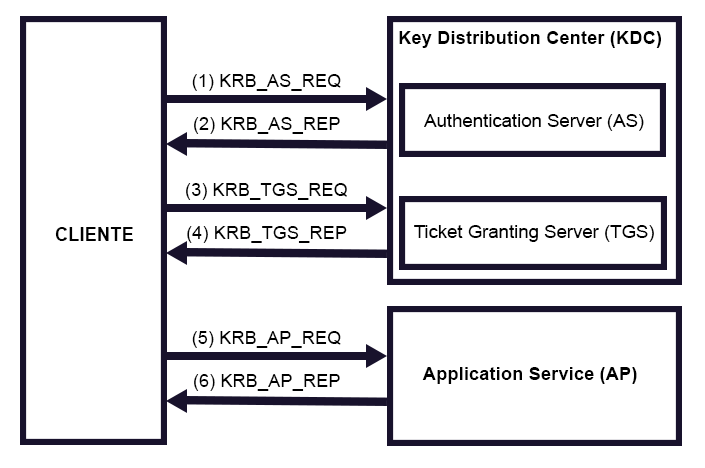
\includegraphics[width=16cm]{Kerberos.png}
\end{center}
\caption{Protocolo de autenticación Kerberos.}
\label{Kerberos}
\end{figure}

\begin{enumerate}

\item En primer lugar, el cliente envía una petición de autenticación al servidor KDC a través del paquete \textbf{KRB\_AS\_REQ}. El objetivo de este paquete es iniciar la comunicación y transmitir las credenciales del usuario a autenticar. Para ello se transmite la siguiente información:

\textbf{- Timestamp:} Sirve para evitar ataques de replay. Está firmado con la clave NTLM del cliente.\\
\textbf{- Username:} Información sobre el nombre del usuario que se está autenticado.\\
\textbf{- Service Principal Name (SPN)~\cite{Capitulo3:SPN}:} Indicador único de la instancia del servicio asociado a la cuenta krbtgt. \\
\textbf{- Nonce:} Número aleatorio generado por el usuario. \\

\item El {\it Authentication Server (AS)} recibe el paquete anterior y procede a la autenticación. Para ello busca el nombre de usuario en la base de datos del KDC y utiliza el hash de la contraseña almacenada para descifrar el timestamp, si no se produce ningún error al descifrar y el timestamp coincide con la hora actual (con un desfase máximo de 5 minutos) la autenticación se completa correctamente. \\

Una vez autenticado el usuario, el AS prepara el paquete a enviar denominado \textbf{KRB\_AS\_REP}. Este paquete contiene la siguiente información:

\textbf{- Username:} Información sobre el nombre del usuario que se está autenticado.\\
\textbf{- Datos cifrados:} Información cifrada con la clave del usuario que incluye: Nombre del usuario, clave de sesión, fecha de expiración de la sesión, SPN y el nonce enviado por el cliente previamente. \\
\textbf{- Ticket TGT:} Ticket cifrado con la clave del KDC. El ticket incluye: Nombre del usuario, clave de sesión, fecha de expiración del ticker TGT y PAC. \\

\item Una vez autenticado y en disposición del TGT. Para poder utilizar un servicio es necesario obtener un TGS. Para ello, el usuario envía un paquete \textbf{KRB\_TGS\_REQ} con la siguiente información:

\textbf{- SPN:} Indicador único de la instancia del servicio asocido a la cuenta krbtgt. \\
\textbf{- Nonce:} Número aleatorio generado por el usuario. \\
\textbf{- Ticket TGT}
\textbf{- Datos cifrados:} Datos cifrados con la clave del usuario que incluye: Nombre de usuario y timestamp. \\

\item {\it Ticket Granting Server} examina la petición, si esta es correcta envía el paquete \textbf{KRB\_TGS\_REP} con el TGS y la siguiente información:

\textbf{- Username}. \\
\textbf{- Ticket TGS:} Ticket cifrado con la clave del servicio. El ticket incluye: Clave de sesión del servicio, nombre de usuario, fecha de expiración del ticket TGS y PAC. \\
\textbf{- Datos cifrados:} Información cifrada con la clave de sesión que incluye: Clave de sesión del servicio, fecha de expiración del ticket TGS y Nonce enviado previamente.

\item Una vez obtenido el ticket TGS, el usuario podrá presentarlo al servicio correspondiente, para ello debe enviar a dicho servicio el paquete \textbf{KRB\_AP\_REQ} con la siguiente información: 

\textbf{- Ticket TGS}.\\
\textbf{- Datos cifrados:} Información cifrada con la clave de sesión del servicio que incluye: Nombre de usuario y timestamp. \\

\item Por último, el servidor contesta con el paquete \textbf{KRB\_AP\_REP}. Este paquete es opcional y sólo se envía si es necesaaria la autenticación mutua entre el cliente y el servicio. 

\end{enumerate}

